
\begin{figure*}[!t]
\begin{minipage}{.5\linewidth}
\centering
        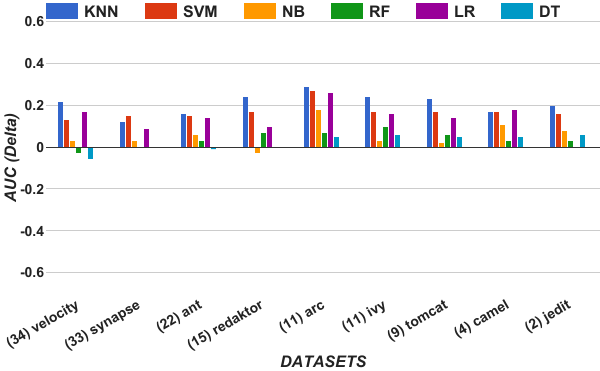
\includegraphics[width=.95\linewidth]{./fig/AUC_untuned.png}
        
  {\bf Figure~\ref{fig:untuned}a:} AUC (pf, recall)
        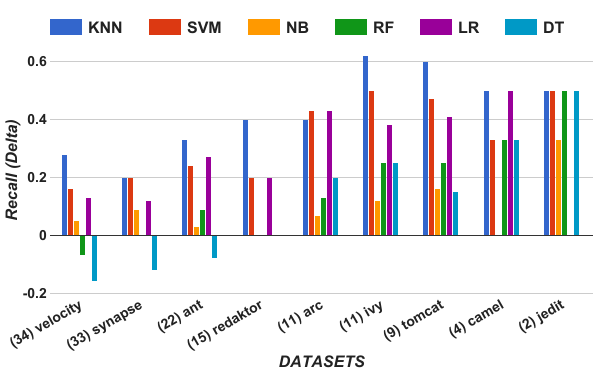
\includegraphics[width=.95\linewidth]{./fig/Recall_untuned.png}
  {\bf Figure~\ref{fig:untuned}c:} Recall
    \end{minipage}%
\begin{minipage}{.5\linewidth}
        \centering
        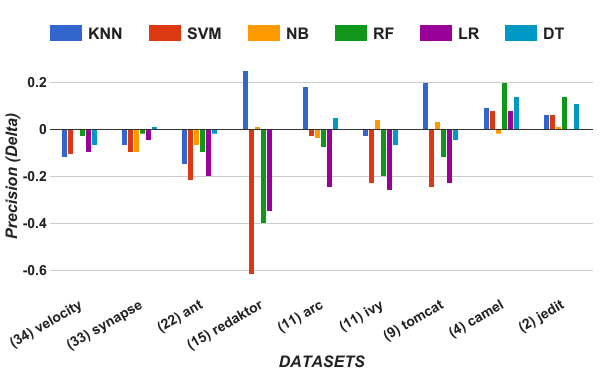
\includegraphics[width=.95\linewidth]{./fig/prec_untuned.png}
  {\bf Figure~\ref{fig:untuned}b:} Precision
        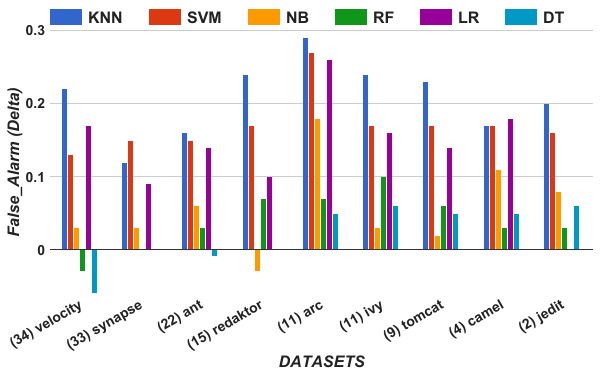
\includegraphics[width=.95\linewidth]{./fig/pf_untuned.png}
  {\bf Figure~\ref{fig:untuned}d:} False Alarm
    \end{minipage}%
    \caption{SMOTE1 improvement over No SMOTE. Legends represent the classifiers mentioned in \tion{classes}}
    \label{fig:untuned}
\end{figure*}

\begin{figure*}[!t]
\begin{minipage}{.5\linewidth}
\centering
        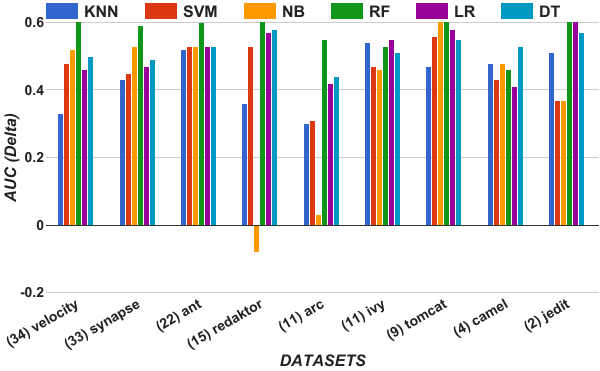
\includegraphics[width=.95\linewidth]{./fig/AUC_tuned.png}
        
  {\bf Figure~\ref{fig:tuned}a:} AUC (pf, recall)
        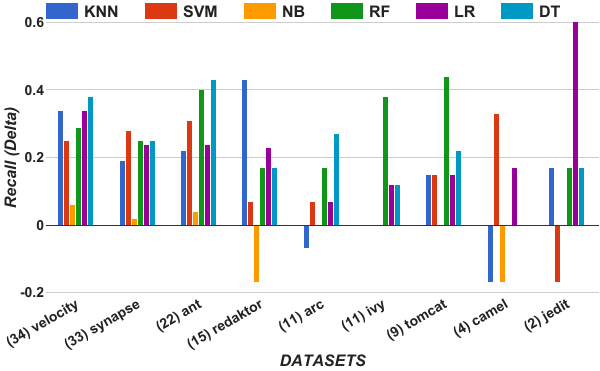
\includegraphics[width=.95\linewidth]{./fig/Recall_tuned.png}
  {\bf Figure~\ref{fig:tuned}c:} Recall
    \end{minipage}%
\begin{minipage}{.5\linewidth}
        \centering
        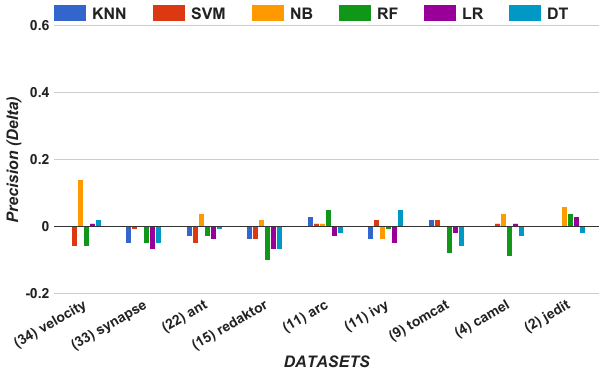
\includegraphics[width=.95\linewidth]{./fig/prec_tuned.png}
  {\bf Figure~\ref{fig:tuned}b:} Precision
        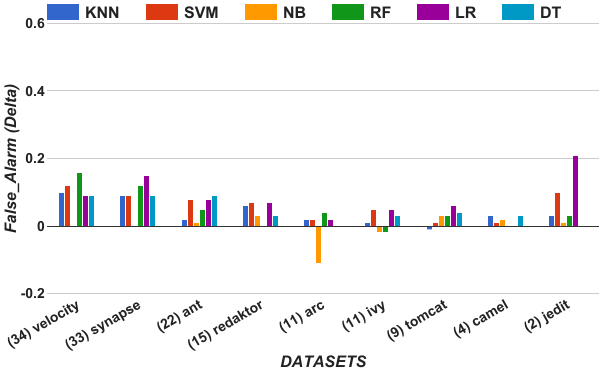
\includegraphics[width=.95\linewidth]{./fig/pf_tuned.png}
  {\bf Figure~\ref{fig:tuned}d:} False Alarm
    \end{minipage}%
    \caption{SMOTE2 improvement over SMOTE1. Legends represent the classifiers mentioned in \tion{classes}.}
    \label{fig:tuned}
\end{figure*}

\section{Results}
\label{sect:results}

\subsection{\textbf{RQ1: Is standard ``off-the-shelf'' SMOTE1 preprocessing method important for defect prediction?}}
Figure~\ref{fig:untuned} represents the improvement of SMOTE1 (median value) against the No SMOTE (median value) results and Figure~\ref{fig:tuned} represents the improvement of SMOTE2 (median value) against SMOTE1 (median value) results. Each figure contains subfigures for all our 4 evaluation measures (mentioned in \tion{measure}) compared with 6 learners (mentioned in \tion{classes}). 



For subfigures (AUC, Recall and Precision) in each Figure~\ref{fig:untuned} and \ref{fig:tuned}:
\bi
\item 
{\em Larger} y-values
are {\em better} 
\item
If the y-value goes {\em negative}, then the corresponding learner performs {\em worse}. 
\ei
For the false alarms, the
plots must be interpreted differently:
\bi
\item
{\em Larger} y-values are {\em worse};
\item
If the y-value goes {\em positive} then
the corresponding leaner
performs {\em worse}.
\ei
Note that, using SMOTE1 on KNN, SVM,
LR (linear regression) often
leads to much larger false alarm increases.
On the other hand,   NB
and RF have much smaller
increase in false alarm.

In these figures, the
X-axis shows all 9 data sets in the decreasing percentage of defective classes from left to right. The corresponding percentage of minority class (in this case, defective class) is written beside each data set. Note that:
\bi
\item
According to the proponents
of SMOTE, SMOTE's improvements should
{\em increase} as we move left to right
across those plots.
\item
No such trend exists in our results for
AUC, precision or false alarms.
\item
For recall, looking left-to-right across
Figure~\ref{fig:untuned}c, we can see
more large positive increases on the
right-hand-side than the left.
\ei
% Based on these results,  we can best recommend SMOTE1 when:
% \bi
% \item Trying to improve recall
% for imbalanaced data sets;
% \item
% Using NB or Random Forests.
% \ei

% For SMOTE2 improvement over SMOTE1 (figure~\ref{fig:tuned}), AUC values are shown in subfigure~\ref{fig:tuned}a. Redaktor data set is selected from X-axis, and yellow bar represents NB which corresponds to about $-0.08$ AUC value. This denotes that NB performed worse by tuning the parameters of SMOTE1. The original parameter settings of SMOTE1 worked the best. On the other hand for the same data set, KNN (which is represented in dark blue bar) shows the AUC value of $0.35$. This shows KNN outperformed the ``off-the-shelf'' SMOTE1 when tuned using DE.



% By looking at the results of AUC from figure~\ref{fig:untuned}a, only 4 bars are negative, and rest all the remaining 50 bars (in total 9 data sets with 6 learners in each) have  positive effect by using SMOTE1 as a preprocessing method. We are seeing a maximum improvement of about 30\%. These improvements are quite modest as to ignore the importance of SMOTE.

% Results for precision (in figure~\ref{fig:untuned}b), are not much interesting, but the decrease in precision value is not that arduous except for the redaktor data set. Though we will not recommend using SMOTE whenever we want higher precision value. Since precision is decreased using SMOTE, it was expected to have increased false alarm \cite{menzies2007problems} and the same is observed from figure~\ref{fig:untuned}d. There is an increase in error among false positives but the increase is very minimal.

% As for recall (figure~\ref{fig:untuned}c), only 4 bars are negative, and rest all the remaining 50 bars (in total 9 data sets with 6 learners in each) have positive effect by using SMOTE1. We are seeing a maximum improvement of about 60\%. These improvements are quite steep as to ignore the importance of SMOTE at any point for any learner. It is also observed that performance keeps increasing as target class becomes more minor and minor. This is what was expected after applying SMOTE to imbalance data sets.

\noindent
Summarizing the above:
\begin{lesson1}
We can recommend SMOTE1 for improving recall, and modest improvements in AUC. But  SMOTE1 adversely effect
precision.
\end{lesson1}

\subsection{\textbf{RQ2: Can tuning SMOTE1 achieve better results?}}

Figure~\ref{fig:tuned} shows the results
after applying SMOTE2. All these
plots show the {\em delta} between
the SMOTE1 results and those of SMOTE2.
As before, {\em positive}  values
are better for AUC, recall and precision
wile {\em negative} values are better for false alarms.

The benefit of SMOTE2's tunings are clearly evident in the AUC results of  Figure~\ref{fig:tuned}a:
all learners show large performance improvements. 
Better yet,  as
shown in
Figure~\ref{fig:tuned}b, and Figure~\ref{fig:tuned}d, SMOTE2 does
not adversely effect false alarm and precision.

SMOTE2's benefits for recall are not very
strong (and seem to be strongest for the more balanced data sets on the left-hand-side of Figure~\ref{fig:tuned}c)
but are rarely negative.




% results are dramat
% Now when we look at the results of AUC from figure~\ref{fig:tuned}a, only 1 bar is negative, and rest all the remaining 53 bars (in total 9 data sets with 6 learners in each) have  positive effect after when we tune the parameters of SMOTE1. We are seeing a maximum improvement of about 70\% and on an average 50\% for each learner in all data sets. These improvements are quite steep in nature and just to remind you that these results are improvement over SMOTE1. If we combine the results, then we can surely say to tune the parameters of SMOTE1 and train using any learner, we will get atleast 100\% improvement in most cases.

% We are seeing the similar trend of results for precision (in figure~\ref{fig:tuned}b), just like in Figure~\ref{fig:untuned}b, that even after tuning for precision, we are not seeing much improvement. Though we definitely improved precision slightly than SMOTE1 but the increment is not that large to recommend SMOTE2 or SMOTE1. And even after trying to minimise the false alarm (figure~\ref{fig:tuned}d) value, DE could not find a good parameter setting.

% As for recall (figure~\ref{fig:untuned}c), only 5 bars are negative, and rest all the remaining 49 bars (in total 9 data sets with 6 learners in each) have either positive effect or no effect after tuning. We are seeing a maximum improvement of about 65\% but the average improvement is close to 15\% for each classifiers in all data sets. But these improvements combined with SMOTE1 suggest that we should always tune SMOTE1 whenever the goal is to achieve higher recall.
In summary:

\begin{lesson1}
    For defect data, SMOTE2  
 offers   some  improvements over SMOTE1 for recall
 and dramatic improvements for AUC (pf, recall) without damaging precision or false
 alarm.
\end{lesson1}

Overall, in  Figure~\ref{fig:tuned},
there are very few negative results
(except in precision, where the negatives
are very small). That is, there
seems little to be lost using SMOTE2
but much to gain (e.g. the large AUC improvements).
Based on these results, we strongly
recommend SMOTE2 for handling unbalanced
data sets.

\begin{figure*}[!t]
    \centering
    \begin{minipage}{.33\textwidth}
        \captionsetup{justification=centering,singlelinecheck=off}
        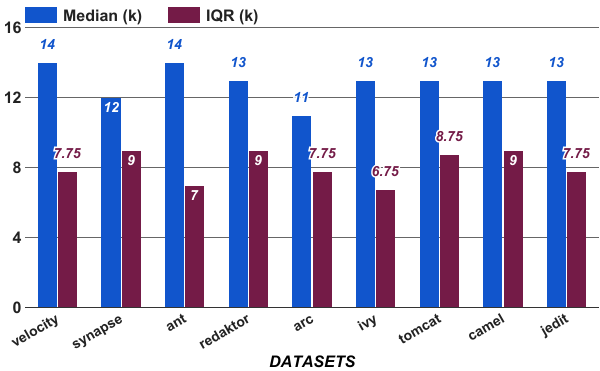
\includegraphics[width=.95\linewidth]{./fig/k.png}
        \caption{Data sets vs Parameter ($k$) variation}
        \label{RQ3:k}
    \end{minipage}%
    \begin{minipage}{.33\textwidth}
        \captionsetup{labelsep=space,justification=centering,singlelinecheck=off}
        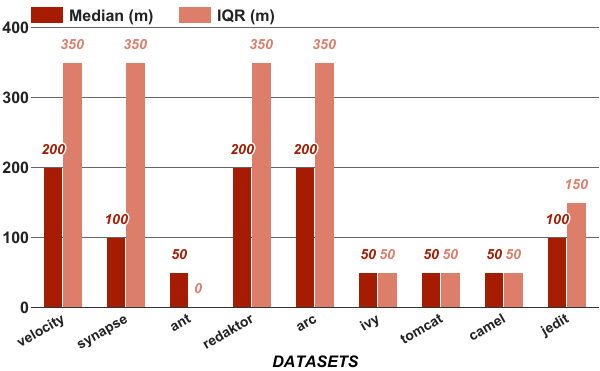
\includegraphics[width=.95\linewidth]{./fig/m.png}
        \caption{Data sets vs Parameter ($m$) variation}
        \label{RQ3:a}
    \end{minipage}
    \begin{minipage}{.33\textwidth}
        \captionsetup{labelsep=space,justification=centering,singlelinecheck=off}
        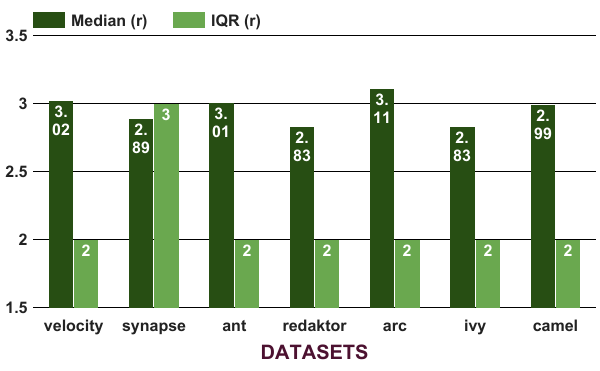
\includegraphics[width=.95\linewidth]{./fig/r.png}
        \caption{Data sets vs Parameter ($r$) variation}
        \label{RQ3:b}
    \end{minipage}
\end{figure*}

\subsection{\textbf{RQ3: Do different data sets
      need different configurations with SMOTE2?}}

Figures \ref{RQ3:k}, \ref{RQ3:a}, and \ref{RQ3:b} show the results of tuning for each data set when recall is considered as evaluation goal. These parameter settings are found by each learner for that data set.
On display in each set of vertical bars are
the median values generated across 15 evaluations.
Also, shown are
the inter-quartile range (IQR) of those tunings (the IQR is the 75th-25th percentile values and is a non-parametric measure of variation
around the median value). Note that in Figure \ref{RQ3:a}, IQR=0 for  ant data set where tuning
          always converged on the same final value.

  These figures
show how tuning selects the different ranges  of
parameters.
Some of the above numbers are far from the standard values; e.g. Chawla et al.~\cite{chawla2002smote} recommend using $k=5$ neighbors yet in our data sets, best results were seen using $k \approx 13$. On other hand it was suggested to use $m=900$ by ~\cite{pears2014synthetic}.
Clearly,
best results from tuning
vary with each data set.

Clearly:
\begin{lesson1}
    DE finds different ``best'' parameter settings for SMOTE2 for different data sets.
\end{lesson1}
 That is,  reusing tunings  suggested  by  any other  previous study  for any data set is \underline{{\em not}} recommended. Instead,  it is better to
      use  automatic  tuning  methods  to find the best tuning parameters for the current data set.
      

\begin{figure}[!t]
  \captionsetup{justification=centering}
  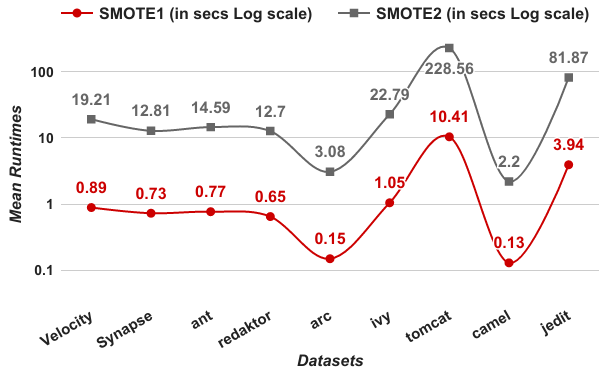
\includegraphics[width=\linewidth]{./fig/runtimes.png}
  \caption{Data sets vs Runtimes}
  \label{runtime}
\end{figure} 

\subsection{\textbf{RQ4: Is tuning impractically slow?}}

Search-based SE methods can be very slow. Wang et al.~\cite{wang2013searching} once needed 15
years of CPU time to find and verify the tunings required for software
clone detectors. Sayyad et al.~\cite{sayyad2013scalable} routinely used
$10^6$ evaluations (or more) of their models in order to extract
products from highly constrained product
lines. Hence, before recommending any
search-based method, it is wise to consider the runtime cost of that
recommendation.

To understand our timing results, recall that SMOTE2 uses
Algorithm~1. Based on the psuedocode
shown above, our pre-experimental expectation is that
tuning will be three to fives times slower than not tuning.  
Figure~\ref{runtime} checks if that theoretical
holds true in practice. Shown in circle and square markers are the
  runtimes required to run SMOTE1 and SMOTE2 respectively.  The
  longer runtimes (in square) include the times required for DE to find
  the tunings. Overall, tuning slows down the training by a factor of up to
  five (which is very close to our theoretical prediction).

\begin{lesson1}
    Tuning with DE makes training four to five times slower, but the improvements which we get for AUC and recall is quite advantageous.
\end{lesson1}
